\documentclass[12pt]{article}

\usepackage{fullpage}
\usepackage{multicol,multirow}
\usepackage{tabularx}
\usepackage{listings}
\usepackage[utf8]{inputenc}
\usepackage[russian]{babel}
\usepackage{graphicx}
\usepackage{csquotes}

\begin{document}

\begin{titlepage}

    \begin{center}

        \bfseries
        {\small Московский авиационный институт\\ 
        (национальный исследовательский университет)}

        % \vspace{48pt}
        {\small Факультет информационных технологий и прикладной 
        математики}
        
        % \vspace{36pt}
        {\small Кафедра вычислительной математики и программирования}
        
        \vspace{8cm}
        {\Large Лабораторная работа \textnumero 1 по курсу} 
        \enquote{\Large Компьютерная графика}
        
    \end{center}
    
    \vspace{84pt}
    \begin{flushright}
        \begin{tabular}{rl}
            Студент: & Е.Ю. Юрков \\
            % Преподаватель: &  \\
            Группа: & М80-312Б-22 \\
            Дата: & \\
            Оценка: & \\
            Подпись: & \\
        \end{tabular}
    \end{flushright}
    
    \vfill
    
    \begin{center}
        
        \bfseries
        Москва, \the\year
    
    \end{center}

\end{titlepage}

% \section*{Лабораторная работа №1\, по курсу компьютерной графики: Основы 2D-графики и трансформаций}

% Выполнил студент группы М8О-312Б-22 МАИ \textit{Юрков Евгений}.

\subsection*{Цель лабораторной работы}

В данной лабораторной работе вам предстоит научиться работать с графическим API для
отрисовки 2D-примитивов, освоить основные 2D-трансформации (перемещение,
масштабирование, поворот) и изучить алгоритмы построения 2D-кривых.

\subsection*{Задача}

\textbf{Вариант 7. Отрисовка многоугольника с интерполяцией}

Постройте многоугольник с 6-ю вершинами.
Реализуйте перемещение всех вершин одновременно с помощью матричных операций.
Добавьте интерполяцию между начальной и конечной позицией многоугольника для
плавного движения.
Дополнительно: Реализуйте циклическую анимацию, при которой многоугольник меняет
свою форму и возвращается в исходное состояние.

% \newpage
\subsection*{Метод решения}

Для выполнения поставленной задачи было принято решение использовать
язык программирования C++ и библиотеку SFML. Была реализована циклическая анимация,
в которой шестиугольник перемещается из центра экрана в случайную точку на границе экрана,
при этом растягиваясь по оси x.

Для построения шестиугольника использовался класс \texttt{sf::CircleShape} с 6 вершинами.

Чтобы шестиугольник плавно перемещался между двумя точками была реализована интерполяция.
В каждой итерации цикла изменялся коэффициент интерполяции: 
$$t = min(t + {\frac{interval}{movetime}}, 1)$$
Где $interval$ - время, прошедшее между кадрами, $movetime$ - время,
за которое фигура должна совершить движение между точками в секундах (задаётся заранее).
Для вычисления текущей позиции фигуры используется формула:
$$p = start \cdot (1 - t) + end \cdot t$$
Где $start$, $end$ - начальная и конечная позиции соответственно.

Также на каждой итерации цикла вычисляется коэффициент растяжения фигуры,
для изменения её формы (дополнительное задание).

Все операции над фигурой, такие как перемещение и масштабирование, производились
с помощью матрицы трансформаций, представленной классом \texttt{sf::Transform}.
Трансформация применялась к шестиугольнику в каждом кадре функцией \texttt{window.draw(hexagon, matrix)}.

% \textbf{Результат работы программы}.
\subsection*{Результат работы программы}

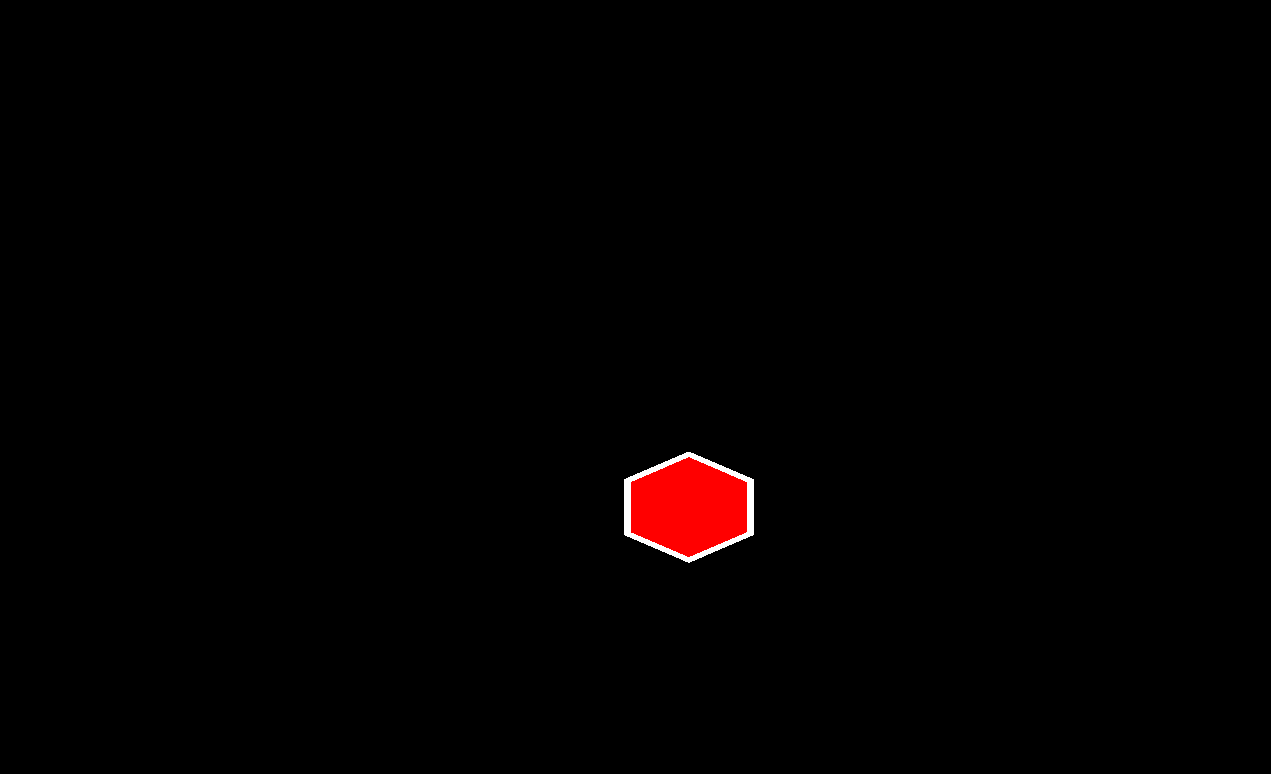
\includegraphics[width=15cm]{demo.png}

% \newpage
\subsection*{Выводы}

В процессе выполнения данной лабораторной работы я изучил основы 2D-графики
и трансформаций с использованием библиотеки SFML на C++.
Используя матрицы трансформаций я разобрался,
как работает геометрическая трансформация в компьютерной графике.
Я узнал, что такое интерполяция, и реализовал плавное перемещение фигуры
через неё, что добавило анимации естественности и гибкости.

Сложности возникли при правильной отрисовке
и трансформации 2D-объектов, поскольку потребовалось
точное управление координатами шестиугольника.
Работа с SFML также потребовала более глубокого изучения документации
для правильного использования её возможностей в графической части и анимации.

Полученные знания могут быть полезны при разработке простых 2D-игр
или визуализации данных, где важны анимации и преобразования объектов.
Опыт работы с трансформациями и базовыми анимационными техниками также будет
полезен для будущих работ, где требуется визуальная интерактивность или работа с графикой.

\end{document}